\listfiles
\documentclass{article}
\author{Arya Stark}

\usepackage{amsmath}
\usepackage{amssymb}
\usepackage{mathtools}
\usepackage{listings}
\usepackage{float}
\usepackage{tikz}
\usepackage{tikz,fullpage}
\usepackage{tkz-graph}
\usepackage[position=top]{subfig}
\usepackage{graphicx}

\DeclarePairedDelimiter\floor{\lfloor}{\rfloor}
\DeclarePairedDelimiter\ceil{\lceil}{\rceil}
\DeclareMathOperator{\cl}{cl}
\DeclareMathOperator{\E}{E}
\def\Z{\mathbb{Z}}
\def\N{\mathbb{N}}
\def\R{\mathbb{R}}
\def\Q{\mathbb{Q}}
\def\K{\mathbb{K}}
\def\T{\mathbb{T}}
\def\B{\mathcal{B}}
\def\XX{\mathfrak{X}}
\def\YY{\mathfrak{Y}}
\def\AA{\mathfrak{A}}
\def\ZZ{\mathfrak{Z}}
\def\BB{\mathcal{B}}
\def\UU{\mathcal{U}}
\def\MM{\mathcal{M}}
\def\M{\mathfrak{M}}
\def\l{\lambda}
\def\L{\Lambda}
\def\<{\langle}
\def\>{\rangle}

\usepackage[a4paper,margin=1in]{geometry}

\setlength{\parindent}{0cm}
\setlength{\parskip}{1em}

\title{Virtual Channels and Rebalancing in State Channel Networks}
\date{}

\begin{document}
\maketitle

\section*{Introduction}

This research note was written because there are some unsolved problems in designing state channel networks that are not well-known or being worked on. These problems reveal themselves when we consider how to build channel networks capable of expressing agents' preferences over network topology (payment capacity) and capital costs, and minimizing blockchain fees.

\section*{Relevant Prerequisite Literature}

This section goes through relevant existing literature. Note that even if you know all this, many definitions will be used in later sections.

\subsection*{Ball-and-bead model of PCN}

In this model, edges represent two-party channel between the endpoints, and a party's balance within the channel is represented by beads near to them.

\begin{center}
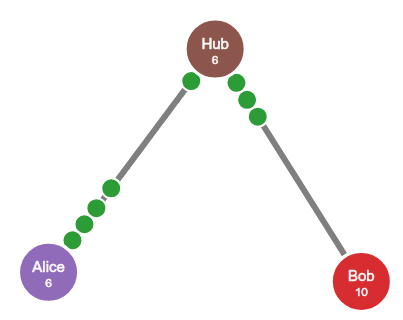
\includegraphics[scale=0.4]{beads.png}
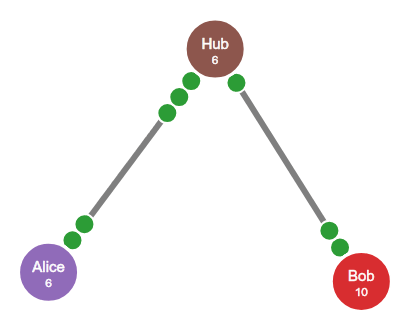
\includegraphics[scale=0.4]{beads2.png}
\end{center}

This shows Alice sending Bob 2 beads via Hub. The remaining capacity along this path is $\min(2,1) = 1$.

\subsection*{Rebalancing}

We say that two channel networks are value-equivalent if the set of agents is the same and each agent owns the same. A channel network is rebalanced when it transitions into a value-equivalent state. This transition can include on-chain transactions or not. In the following on-chain rebalance, Bob increases the capacity of the Bob $\to$ Alice link.

\begin{center}
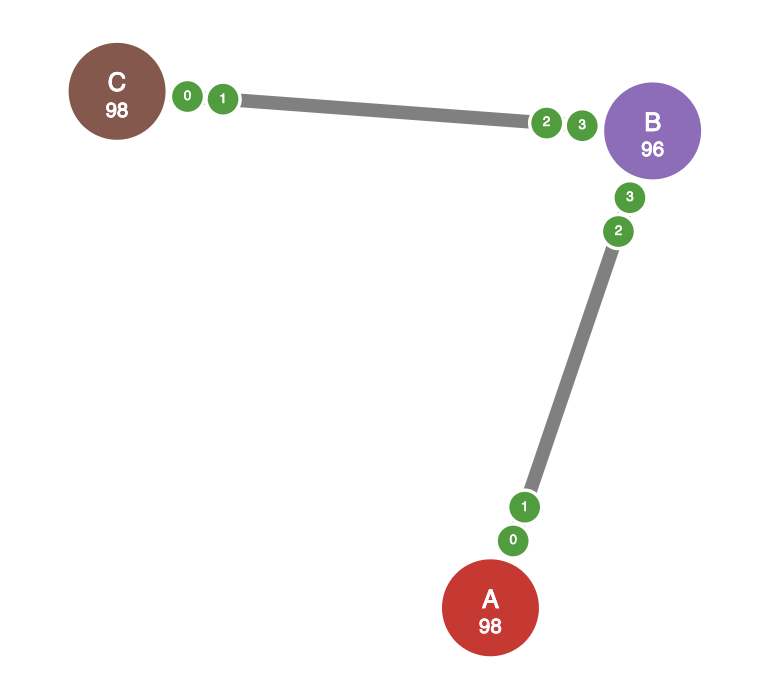
\includegraphics[scale=0.4]{on-chain-rebalancing-1.png}
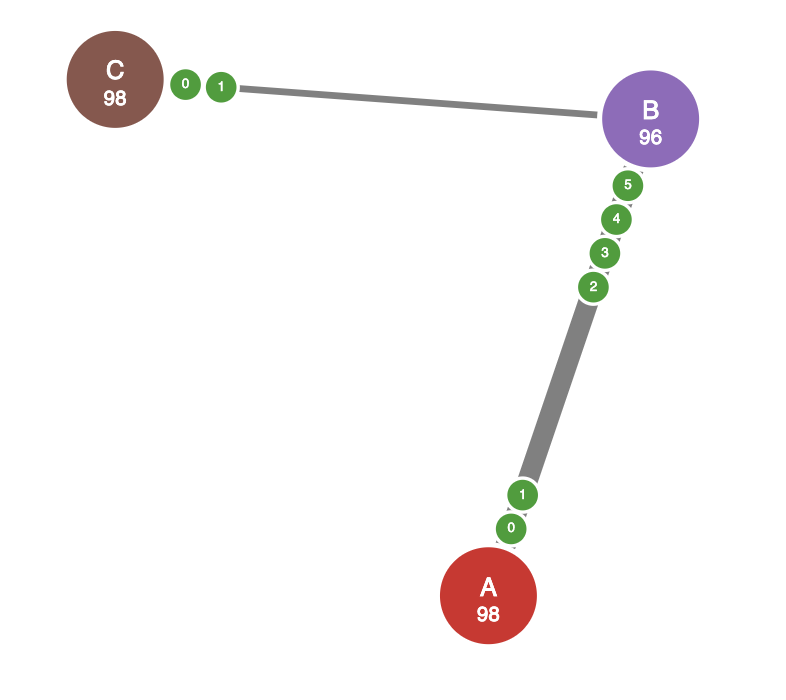
\includegraphics[scale=0.4]{on-chain-rebalancing-2.png}
\end{center}

The following is an example of a rebalance that does not require on-chain transactions.

\begin{center}
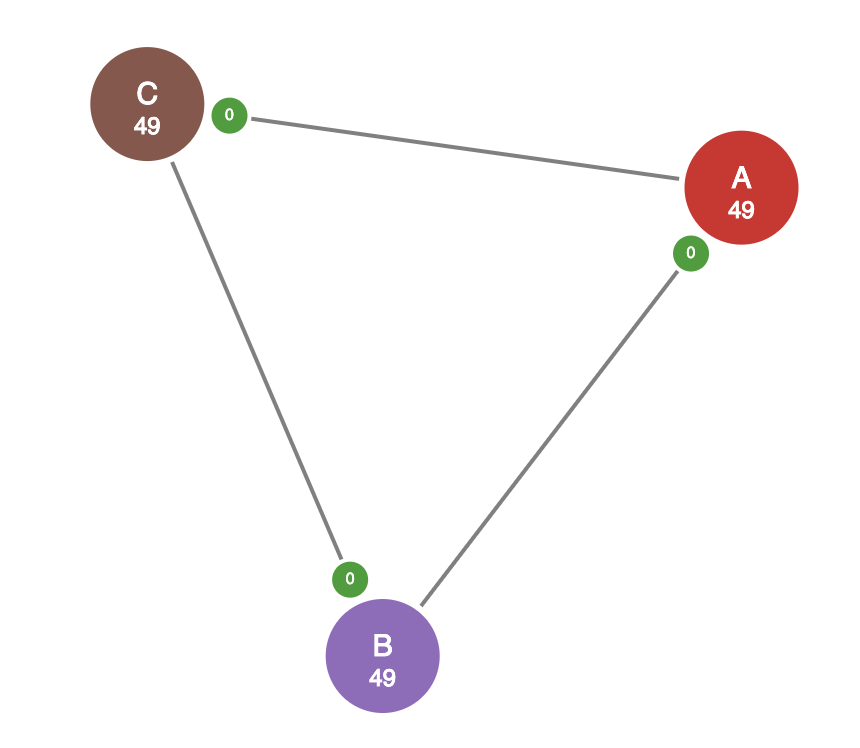
\includegraphics[scale=0.4]{off-chain-rebalancing-1.png}
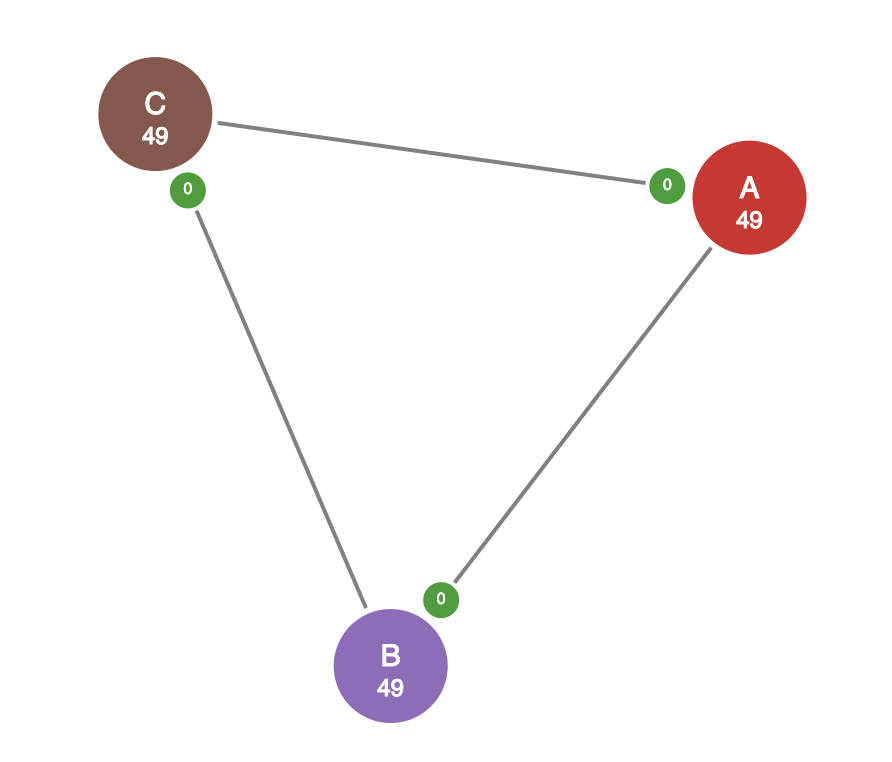
\includegraphics[scale=0.4]{off-chain-rebalancing-2.png}
\end{center}

Are off-chain rebalances sufficient? In general, no.

% TBW: define a $a,b$-flow, apply max-flow-min-cut theorem, etc.

% Note some assumptions implicitly made when applying this theorem: the max flow might requrie very global knowledge to compute.

% Fun exercise! A self-payment is a special type of off-chain rebalance. Show that any rebalance can be expressed as a series of self-payments.

\subsection*{Time-based lockup}

There are two ways that intermediaries can structure agreements-to-route. They can agree to route a single payment. When that payment completes successfully, the balances change and they are free of any further commitments. The second way is to agree to lock up funds for a certain period of time, creating a ``virtual channel". The balances in the virtual channel can be updated instantly and many times without the intermediary's participation or knowledge. At the end of the lockup time, the final balances in the virtual channel are agreed to and we update the direct channel balances as though a single set of routed balance updates (routed payments) was made.

\subsection*{Ejection}

There is an upper bound on the fee that the intermediary can charge, since any virtual channel can be transformed into a direct channel (i.e. it can be ``ejected") by some on-chain transactions, without disrupting the internal state of the virtual channel. Here is an example. Suppose we have this system of direct channels. (Note: we switch to labelling edges by their endpoint balances rather than using beads, due to limitations of latex).

\begin{figure}[H]
    \centering
    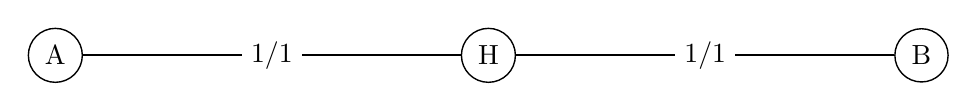
\begin{tikzpicture}[scale=2.75]
        \GraphInit[vstyle=Normal]
        \Vertex[x=0,y=0]{A}
        \Vertex[x=2,y=0]{H}
        \Vertex[x=4,y=0]{B}
        \Edge[label=$1/1$](A)(H)
        \Edge[label=$1/1$](H)(B)
    \end{tikzpicture}
\end{figure}

Here, a virtual channel between A and B can be formed, with balance one bead for each of them, locking up two beads from H. The channel could be ejected by an on-chain transaction that transfers one bead out of the A-H channel and H-B channel and atomically updating the internal states of them.

\begin{figure}[H]
    \centering
    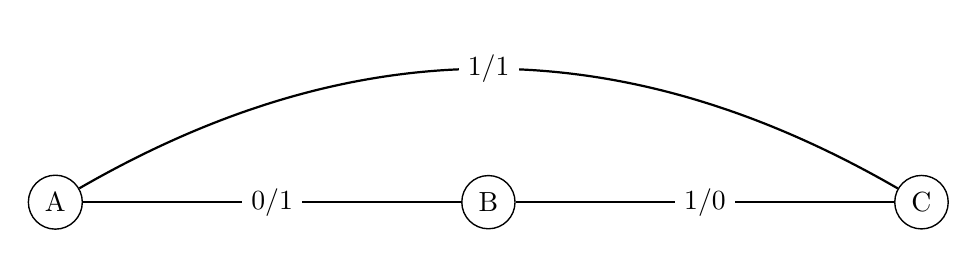
\begin{tikzpicture}[scale=2.75]
        \GraphInit[vstyle=Normal]
        \Vertex[x=0,y=0]{A}
        \Vertex[x=2,y=0]{B}
        \Vertex[x=4,y=0]{C}
        \Edge[label=$0/1$](A)(B)
        \Edge[label=$1/0$](B)(C)
        \Edge[style={bend left},label=$1/1$](A)(C)
    \end{tikzpicture}
\end{figure}

For this reason, thinking of lockups as ``time-based" is not strictly accurate; the costs an intermediary would incur in a channel network is both the cost of re-configuring the capacity graph as well as time-based opportunity cost of having their capital in excess of payments they would want to make anyway in the network (e.g. instead of staking), however both can be avoided by on-chain transactions; the instances where on-chain transactions are avoided and off-chain fees paid instead are therefore some complex subset of transactions in general.

Here is a crude fee scheme that captures some of it this: an intermediary charges some large fee $F_1$ to intermediate a virtual channel, and assumes the responsibility of ejecting the channel; if the virtual channel participants have no further use for it, they negotiate a payment of $F_2$ from the intermediary to close the virtual channel offline. If the on-chain fee is $T$, we should have $0 < F_1 - F_2 < T < F_1$. On/off-chain rebalancing is handeled by an independent protocol.

\subsection*{State Channels}

By allowing beads to be locked into complex applications (e.g. chess, prediction markets) instead of just payments, the need for virtual channels as well as for ejection is even more apparent. Beads can be freed up and re-used within a virtual channel. The time bound for an application might be long or unknown (e.g., we lock beads up in a bet of whether any US Libertarian Party ever wins a House seat in the next 10 years),

\subsection*{Multipath}

TBW

\subsection*{N-Party}

TBW

\subsection*{Subchannels}

TBW

\subsection*{Plasma}

Plasma can be used to fund channels. If all channels are funded by plasma, then rebalancing is a plasma transaction in the normal case, i.e., the entire network can be rebalanced arbitrarily in a single ethereum transaction. I claim that a super-optimized channel network that does not support funding via plasma will be much more expensive than a very suboptimal one that supports funding via plasma.

\section*{Model}

TBW

\section*{Ejection Test Cases}

\subsection*{Symmetric}

\begin{figure}[H]
    \centering
    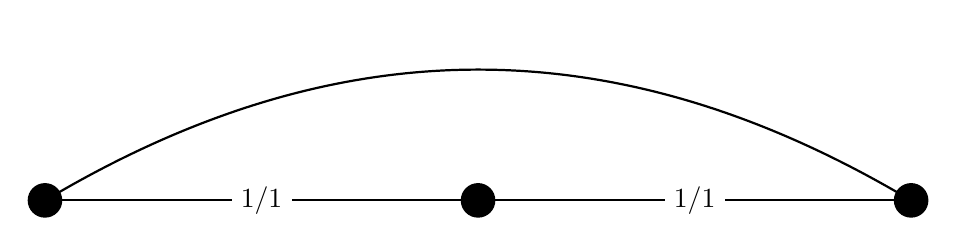
\begin{tikzpicture}[scale=2.75]
        \GraphInit[vstyle=Normal]
        \SetVertexSimple
        \Vertex[x=0,y=0]{A}
        \Vertex[x=2,y=0]{B}
        \Vertex[x=4,y=0]{C}
        \Edge[label=$1/1$](A)(B)
        \Edge[label=$1/1$](B)(C)
        \Edge[style={bend left}](A)(C)
    \end{tikzpicture}
    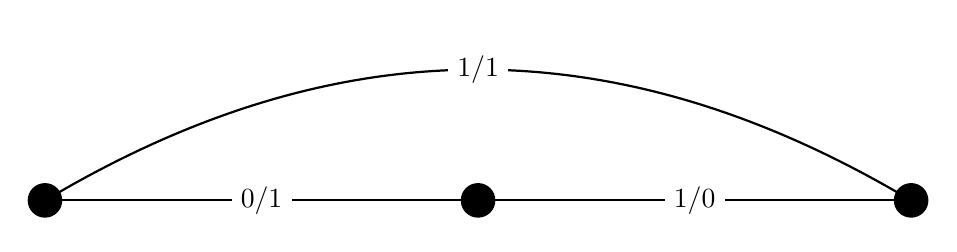
\begin{tikzpicture}[scale=2.75]
        \GraphInit[vstyle=Normal]
        \SetVertexSimple
        \Vertex[x=0,y=0]{A}
        \Vertex[x=2,y=0]{B}
        \Vertex[x=4,y=0]{C}
        \Edge[label=$0/1$](A)(B)
        \Edge[label=$1/0$](B)(C)
        \Edge[style={bend left},label=$1/1$](A)(C)
    \end{tikzpicture}
\end{figure}

Reviewed previously

\subsection*{Asymetric}

\begin{figure}[H]
    \centering
    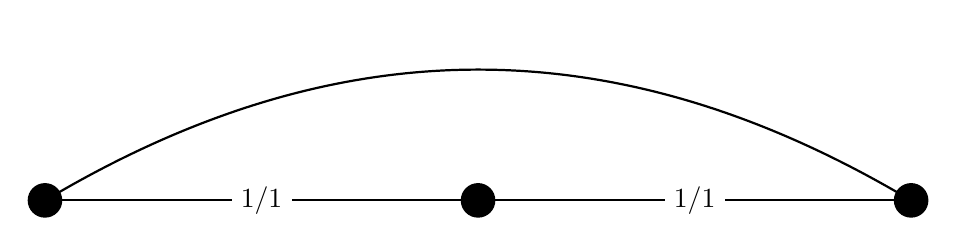
\begin{tikzpicture}[scale=2.75]
        \GraphInit[vstyle=Normal]
        \SetVertexSimple
        \Vertex[x=0,y=0]{A}
        \Vertex[x=2,y=0]{B}
        \Vertex[x=4,y=0]{C}
        \Edge[label=$1/1$](A)(B)
        \Edge[label=$1/1$](B)(C)
        \Edge[style={bend left}](A)(C)
    \end{tikzpicture}
    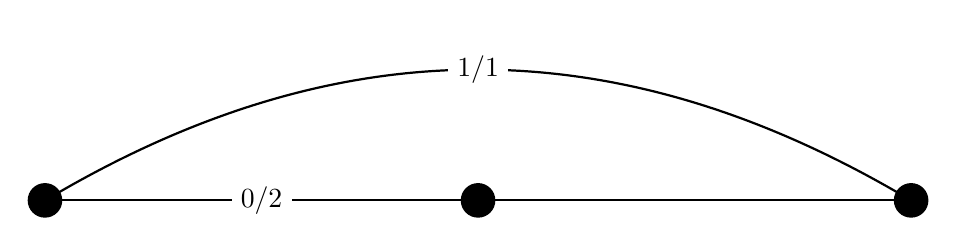
\begin{tikzpicture}[scale=2.75]
        \GraphInit[vstyle=Normal]
        \SetVertexSimple
        \Vertex[x=0,y=0]{A}
        \Vertex[x=2,y=0]{B}
        \Vertex[x=4,y=0]{C}
        \Edge[label=$0/2$](A)(B)
        \Edge(B)(C)
        \Edge[style={bend left},label=$1/1$](A)(C)
    \end{tikzpicture}
\end{figure}

What are the differences between the the assymetric and symmetric ways of ejecting? The symmetric manner might be preferred because it minimal in the number of transactions (1 vs 2). Even if we assume some mechanism to batch two sub-transactions under one (e.g. account abstraction), it is minimal in the number of ERCECOVERS (3 vs 2). On the other hand, the symmetric manner might be preferred for the more ``balanced" resulting capacity graph.

\subsection*{Symmetric Unidirectional}

\begin{figure}[H]
    \centering
    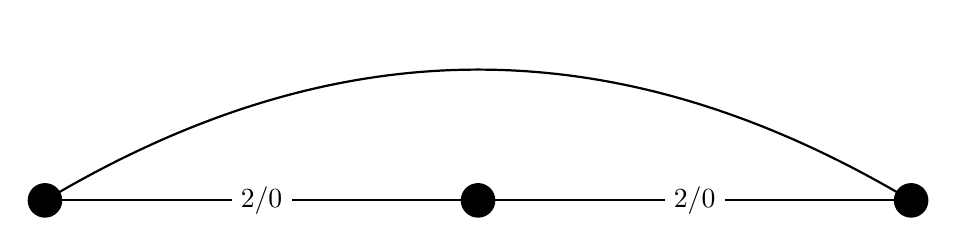
\begin{tikzpicture}[scale=2.75]
        \GraphInit[vstyle=Normal]
        \SetVertexSimple
        \Vertex[x=0,y=0]{A}
        \Vertex[x=2,y=0]{B}
        \Vertex[x=4,y=0]{C}
        \Edge[label=$2/0$](A)(B)
        \Edge[label=$2/0$](B)(C)
        \Edge[style={bend left}](A)(C)
    \end{tikzpicture}
    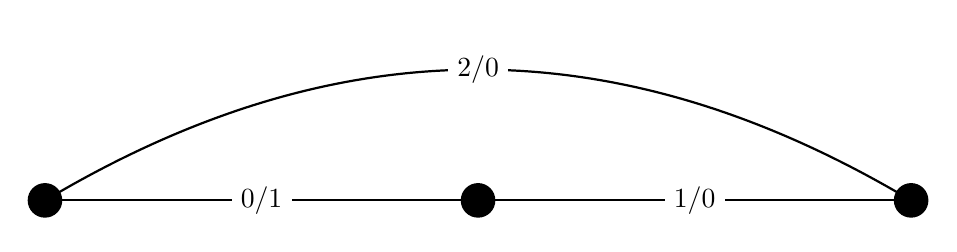
\begin{tikzpicture}[scale=2.75]
        \GraphInit[vstyle=Normal]
        \SetVertexSimple
        \Vertex[x=0,y=0]{A}
        \Vertex[x=2,y=0]{B}
        \Vertex[x=4,y=0]{C}
        \Edge[label=$0/1$](A)(B)
        \Edge[label=$1/0$](B)(C)
        \Edge[style={bend left},label=$2/0$](A)(C)
    \end{tikzpicture}
\end{figure}

\subsection*{Asymmetric Unidirectional 1}

\begin{figure}[H]
    \centering
    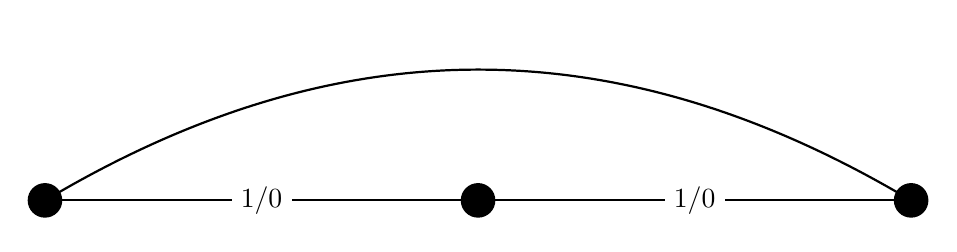
\begin{tikzpicture}[scale=2.75]
        \GraphInit[vstyle=Normal]
        \SetVertexSimple
        \Vertex[x=0,y=0]{A}
        \Vertex[x=2,y=0]{B}
        \Vertex[x=4,y=0]{C}
        \Edge[label=$1/0$](A)(B)
        \Edge[label=$1/0$](B)(C)
        \Edge[style={bend left}](A)(C)
    \end{tikzpicture}
    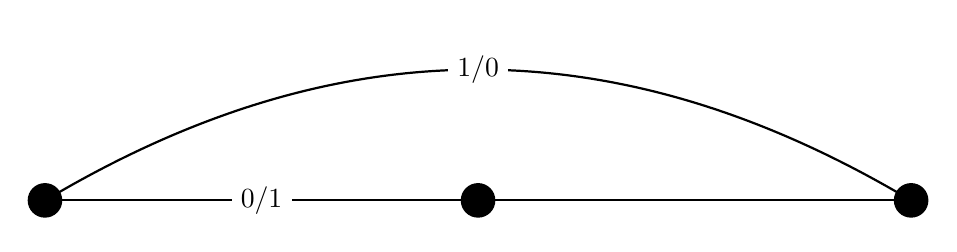
\begin{tikzpicture}[scale=2.75]
        \GraphInit[vstyle=Normal]
        \SetVertexSimple
        \Vertex[x=0,y=0]{A}
        \Vertex[x=2,y=0]{B}
        \Vertex[x=4,y=0]{C}
        \Edge[label=$0/1$](A)(B)
        \Edge(B)(C)
        \Edge[style={bend left},label=$1/0$](A)(C)
    \end{tikzpicture}
\end{figure}

\subsection*{Asymmetric Unidirectional 2}

\begin{figure}[H]
    \centering
    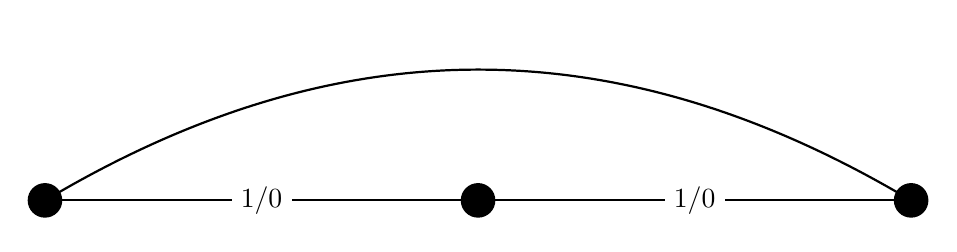
\begin{tikzpicture}[scale=2.75]
        \GraphInit[vstyle=Normal]
        \SetVertexSimple
        \Vertex[x=0,y=0]{A}
        \Vertex[x=2,y=0]{B}
        \Vertex[x=4,y=0]{C}
        \Edge[label=$1/0$](A)(B)
        \Edge[label=$1/0$](B)(C)
        \Edge[style={bend left}](A)(C)
    \end{tikzpicture}
    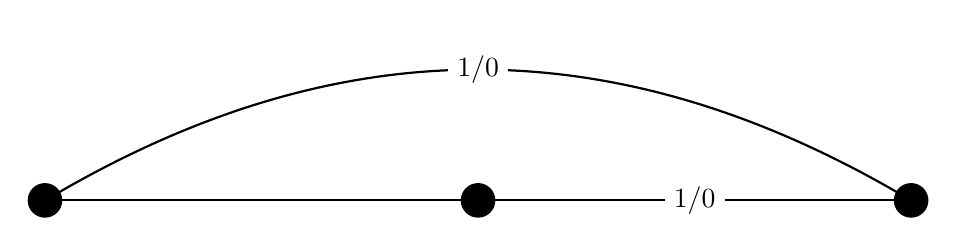
\begin{tikzpicture}[scale=2.75]
        \GraphInit[vstyle=Normal]
        \SetVertexSimple
        \Vertex[x=0,y=0]{A}
        \Vertex[x=2,y=0]{B}
        \Vertex[x=4,y=0]{C}
        \Edge(A)(B)
        \Edge[label=$1/0$](B)(C)
        \Edge[style={bend left},label=$1/0$](A)(C)
    \end{tikzpicture}
\end{figure}

\subsection*{Long-Chain Large-Radius}

\begin{figure}[H]
    \centering
    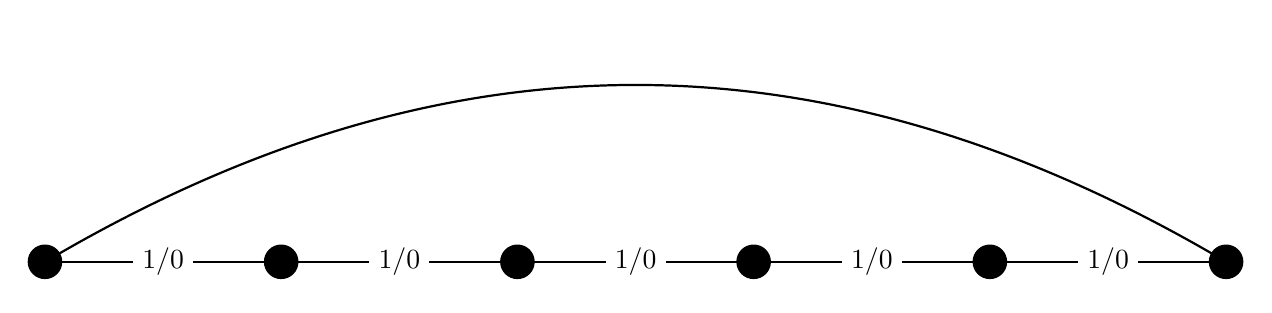
\begin{tikzpicture}[scale=1.5]
        \GraphInit[vstyle=Normal]
        \SetVertexSimple
        \Vertex[x=0,y=0]{A}
        \Vertex[x=2,y=0]{B}
        \Vertex[x=4,y=0]{C}
        \Vertex[x=6,y=0]{D}
        \Vertex[x=8,y=0]{E}
        \Vertex[x=10,y=0]{F}
        \Edge[label=$1/0$](A)(B)
        \Edge[label=$1/0$](B)(C)
        \Edge[label=$1/0$](C)(D)
        \Edge[label=$1/0$](D)(E)
        \Edge[label=$1/0$](E)(F)
        \Edge[style={bend left}](A)(F)
    \end{tikzpicture}
    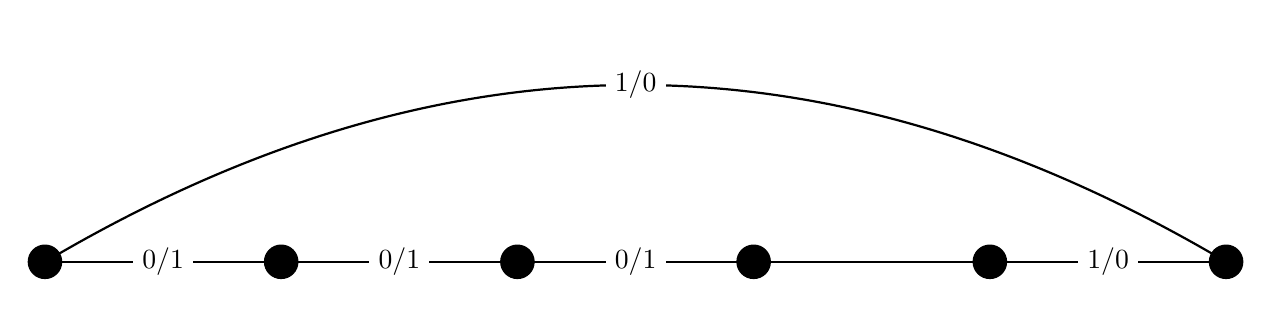
\begin{tikzpicture}[scale=1.5]
        \GraphInit[vstyle=Normal]
        \SetVertexSimple
        \Vertex[x=0,y=0]{A}
        \Vertex[x=2,y=0]{B}
        \Vertex[x=4,y=0]{C}
        \Vertex[x=6,y=0]{D}
        \Vertex[x=8,y=0]{E}
        \Vertex[x=10,y=0]{F}
        \Edge[label=$0/1$](A)(B)
        \Edge[label=$0/1$](B)(C)
        \Edge[label=$0/1$](C)(D)
        \Edge(D)(E)
        \Edge[label=$1/0$](E)(F)
        \Edge[style={bend left},label=$1/0$](A)(F)
    \end{tikzpicture}
\end{figure}

\subsection*{Long-Chain Short-Radius}

\begin{figure}[H]
    \centering
    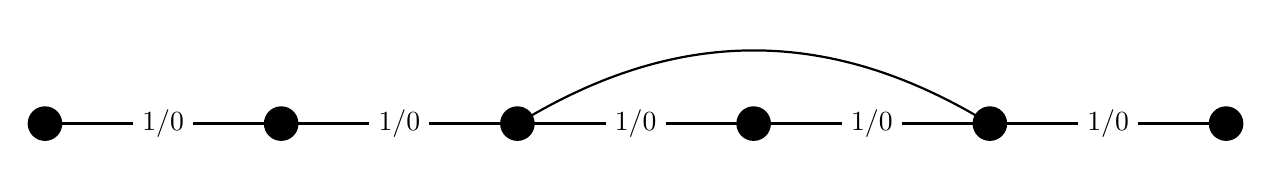
\begin{tikzpicture}[scale=1.5]
        \GraphInit[vstyle=Normal]
        \SetVertexSimple
        \Vertex[x=0,y=0]{A}
        \Vertex[x=2,y=0]{B}
        \Vertex[x=4,y=0]{C}
        \Vertex[x=6,y=0]{D}
        \Vertex[x=8,y=0]{E}
        \Vertex[x=10,y=0]{F}
        \Edge[label=$1/0$](A)(B)
        \Edge[label=$1/0$](B)(C)
        \Edge[label=$1/0$](C)(D)
        \Edge[label=$1/0$](D)(E)
        \Edge[label=$1/0$](E)(F)
        \Edge[style={bend left}](C)(E)
    \end{tikzpicture}
    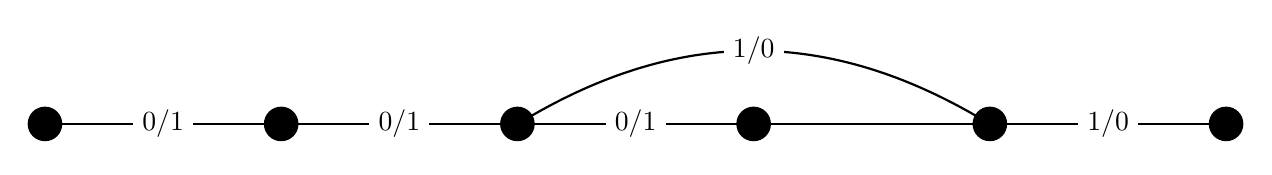
\begin{tikzpicture}[scale=1.5]
        \GraphInit[vstyle=Normal]
        \SetVertexSimple
        \Vertex[x=0,y=0]{A}
        \Vertex[x=2,y=0]{B}
        \Vertex[x=4,y=0]{C}
        \Vertex[x=6,y=0]{D}
        \Vertex[x=8,y=0]{E}
        \Vertex[x=10,y=0]{F}
        \Edge[label=$0/1$](A)(B)
        \Edge[label=$0/1$](B)(C)
        \Edge[label=$0/1$](C)(D)
        \Edge(D)(E)
        \Edge[label=$1/0$](E)(F)
        \Edge[style={bend left},label=$1/0$](C)(E)
    \end{tikzpicture}
\end{figure}

\subsection*{Multipath}

\begin{figure}[H]
    \centering
    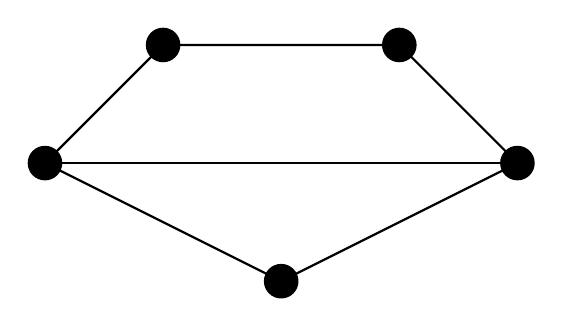
\begin{tikzpicture}[scale=1.5]
        \GraphInit[vstyle=Normal]
        \SetVertexSimple
        \Vertex[x=2,y=0]{D}
        \Vertex[x=0,y=1]{A}
        \Vertex[x=4,y=1]{E}
        \Vertex[x=1,y=2]{B}
        \Vertex[x=3,y=2]{C}
        \Edge(A)(E)
        \Edge(A)(B)
        \Edge(B)(C)
        \Edge(C)(E)
        \Edge(A)(D)
        \Edge(D)(E)
    \end{tikzpicture}
\end{figure}

Balances and ejection to be filled in.

\subsection*{Thanos Star}

New notation: a square node is not a participant, but it means that its neighbours are all connected in a direct channel.

\begin{figure}[H]
    \centering
    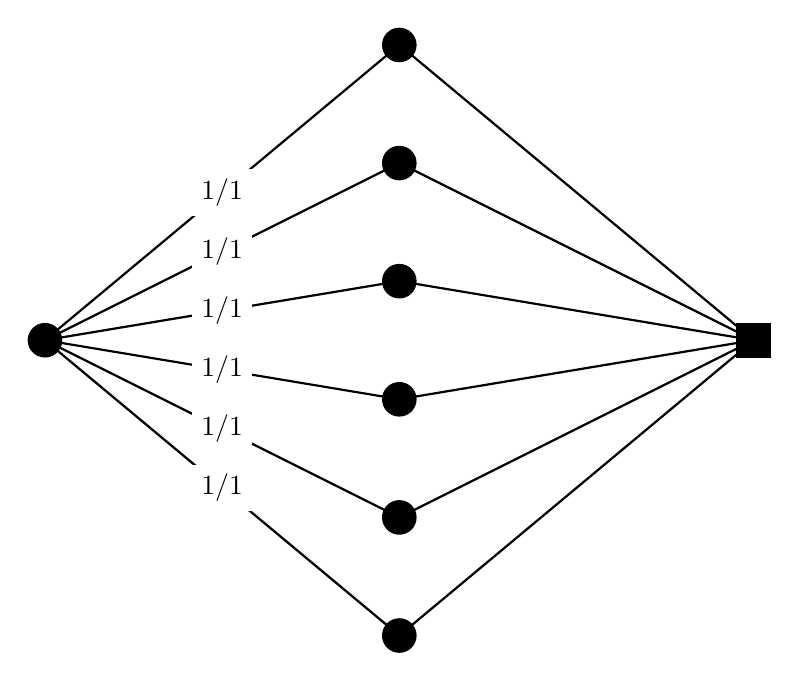
\begin{tikzpicture}[scale=1.5]
        \GraphInit[vstyle=Normal]
        \SetVertexSimple
        \Vertex[x=0,y=2.5]{A}
        \Vertex[x=3,y=0]{B}
        \Vertex[x=3,y=1]{C}
        \Vertex[x=3,y=2]{D}
        \Vertex[x=3,y=3]{E}
        \Vertex[x=3,y=4]{F}
        \Vertex[x=3,y=5]{G}
        \begin{scope}[VertexStyle/.append style = {rectangle}]
        \Vertex[x=6,y=2.5,style={color=red}]{H}
        \end{scope}
        \Edge[label=$1/1$](A)(B)
        \Edge[label=$1/1$](A)(C)
        \Edge[label=$1/1$](A)(D)
        \Edge[label=$1/1$](A)(E)
        \Edge[label=$1/1$](A)(F)
        \Edge[label=$1/1$](A)(G)
        \Edge(H)(B)
        \Edge(H)(C)
        \Edge(H)(D)
        \Edge(H)(E)
        \Edge(H)(F)
        \Edge(H)(G)
    \end{tikzpicture}
\end{figure}

\begin{figure}[H]
    \centering
    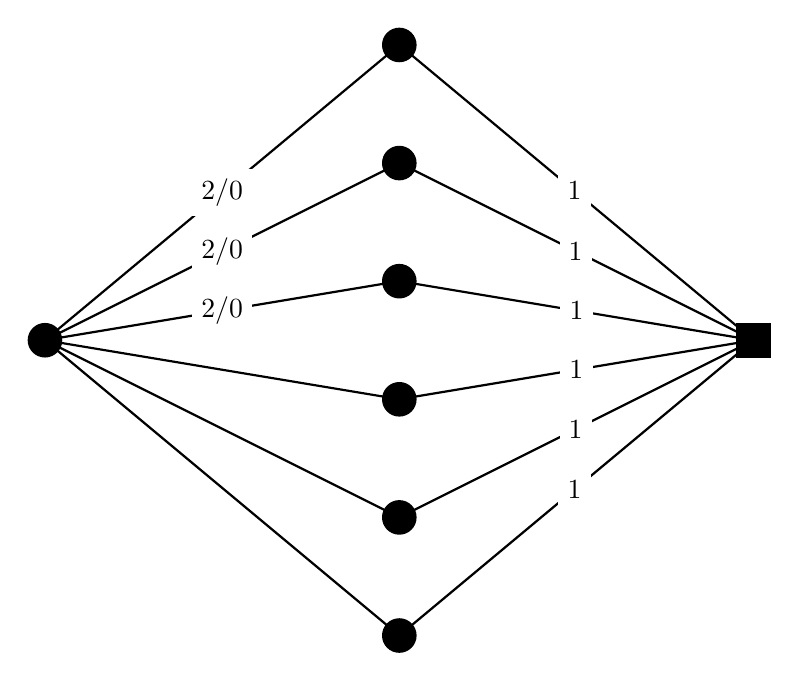
\begin{tikzpicture}[scale=1.5]
        \GraphInit[vstyle=Normal]
        \SetVertexSimple
        \Vertex[x=0,y=2.5]{A}
        \Vertex[x=3,y=0]{B}
        \Vertex[x=3,y=1]{C}
        \Vertex[x=3,y=2]{D}
        \Vertex[x=3,y=3]{E}
        \Vertex[x=3,y=4]{F}
        \Vertex[x=3,y=5]{G}
        \begin{scope}[VertexStyle/.append style = {rectangle}]
        \Vertex[x=6,y=2.5,style={color=red}]{H}
        \end{scope}
        \Edge(A)(B)
        \Edge(A)(C)
        \Edge(A)(D)
        \Edge[label=$2/0$](A)(E)
        \Edge[label=$2/0$](A)(F)
        \Edge[label=$2/0$](A)(G)
        \Edge[label=$1$](H)(B)
        \Edge[label=$1$](H)(C)
        \Edge[label=$1$](H)(D)
        \Edge[label=$1$](H)(E)
        \Edge[label=$1$](H)(F)
        \Edge[label=$1$](H)(G)
    \end{tikzpicture}
\end{figure}

A 6-party virtual channel gets ejected into a 6-party direct channel. This manner of ejecting is minimal in number of transactions.

\section*{Other test cases}

\subsection*{Under-Capacity Three Party Channel}

\begin{figure}[H]
    \centering
    \begin{tikzpicture}[scale=1.5]
        \GraphInit[vstyle=Normal]
        \Vertex[x=0,y=0]{A}
        \Vertex[x=0,y=2]{B}
        \Vertex[x=3,y=1]{H}
        \Vertex[x=6,y=1]{C}
        \Edge[label=$1/0$](A)(H)
        \Edge[label=$1/0$](B)(H)
        \Edge[label=$1/0$](H)(C)
    \end{tikzpicture}
\end{figure}

If A,B,C form a virtual channel through H, they end up in a three-party virtual channel where A can send C one bead, and B can send C one bead, but the two cannot happen at the same time. The challenge is that it is inappropirate to represent this as a three-party channel where A and B's balances are both one.

\subsection*{Self Lock-in}

TBW


\end{document}